\begin{figure*}[p]
\begin{minipage}[t]{.48\textwidth}\vspace{0pt}
\localtablecaption{主结果分数据集核对。每格为同64个输入在三档预算下的成功总数/192。两个数据集的模式完全相同，反映构造语义主导的限制。}\label{tab:network-datasets}
\centering\small
\begin{tabularx}{\columnwidth}{Xrr}
\toprule
策略 & WDBC & Banknote \\
\midrule
词法前五＋路径 & 12/192 & 12/192 \\
MMR 前五＋路径 & 60/192 & 60/192 \\
DPP 前五＋路径 & 60/192 & 60/192 \\
原生元数据最短路径 & 24/192 & 24/192 \\
人工固定流程 & 128/192 & 128/192 \\
全局证据过滤＋最短路径 & 64/192 & 64/192 \\
全局证据风险路径 & 128/192 & 128/192 \\
ECP 完整方法 & 136/192 & 136/192 \\
条件证据前五＋路径 & 90/192 & 90/192 \\
ECP 去版本绑定 & 136/192 & 136/192 \\
\bottomrule
\end{tabularx}

\vspace{8mm}\raggedright\small
主留出只包含128个不同输入，每个数据集64个。表中192为64个输入乘三档预算；两个数据集同样的成功总数不代表192个独立任务，也不能用重复预算缩窄区间。

\medskip
原始记录位置：\texttt{research/skill\_network/results/} 下的 \texttt{prepared-v3}、\texttt{calibration-v2}、\texttt{execution-v2}、\texttt{analysis-v1} 和 \texttt{joint-posthoc-v1}。
公开元数据、执行前选择、worker请求、原始输出和逐项判定分别保存，便于审查是否发生答案泄漏或失败删除。

\medskip
完整复现同时检查原始源文件指纹、开发/留出隔离、逐次选择、全部产物、三档聚合、条件重采样及事后反例。CI复现报告记录了无凭据、无网络及只读边界；它增加实现可移植性证据，不增加科学样本或领域认可。
\end{minipage}\hfill
\begin{minipage}[t]{.48\textwidth}\vspace{0pt}
\centering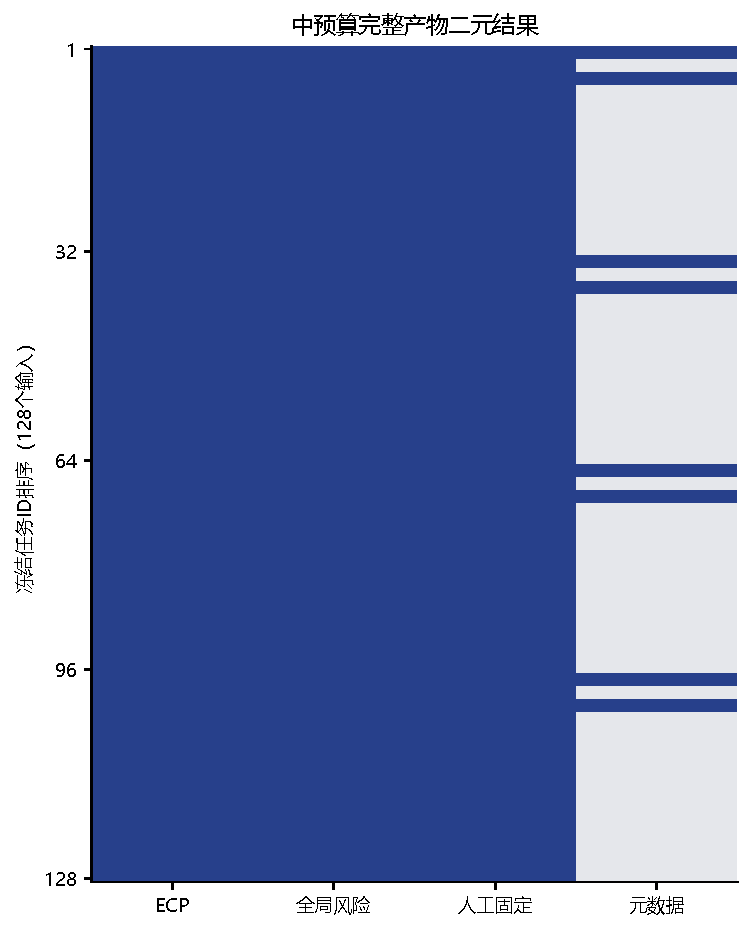
\includegraphics[width=.96\linewidth]{figures/network_binary_matrix.pdf}
\localfigurecaption{中预算128个主输入的二元完整成功矩阵。按冻结ID排序，蓝色为全部检查通过，灰色为失败或弃权；这里只显示四个预定代表策略，全部十策略记录随稿。}
\label{fig:network-matrix}
\end{minipage}
\end{figure*}
